\documentclass[12pt]{report}
\usepackage[utf8]{inputenc}
\usepackage[russian]{babel}
%\usepackage[14pt]{extsizes}
\usepackage{listings}
\usepackage{graphicx}
\usepackage{amsmath,amsfonts,amssymb,amsthm,mathtools} 
\usepackage{pgfplots}
\usepackage{filecontents}
\usepackage{indentfirst}
\usepackage{eucal}
\usepackage{amsmath}
\usepackage{enumitem}
\usepackage{fixltx2e}
\usepackage{float}

\frenchspacing

\usepackage{indentfirst} % Красная строка


%\usetikzlibrary{datavisualization}
%\usetikzlibrary{datavisualization.formats.functions}

\usepackage{amsmath}


% Для листинга кода:
\lstset{ %
language=caml,                 % выбор языка для подсветки (здесь это С)
basicstyle=\small\sffamily, % размер и начертание шрифта для подсветки кода
numbers=left,               % где поставить нумерацию строк (слева\справа)
numberstyle=\tiny,           % размер шрифта для номеров строк
stepnumber=1,                   % размер шага между двумя номерами строк
numbersep=5pt,                % как далеко отстоят номера строк от подсвечиваемого кода
showspaces=false,            % показывать или нет пробелы специальными отступами
showstringspaces=false,      % показывать или нет пробелы в строках
showtabs=false,             % показывать или нет табуляцию в строках
frame=single,              % рисовать рамку вокруг кода
tabsize=2,                 % размер табуляции по умолчанию равен 2 пробелам
captionpos=t,              % позиция заголовка вверху [t] или внизу [b] 
breaklines=true,           % автоматически переносить строки (да\нет)
breakatwhitespace=false, % переносить строки только если есть пробел
escapeinside={\#*}{*)}   % если нужно добавить комментарии в коде
}

\usepackage[left=2cm,right=2cm, top=2cm,bottom=2cm,bindingoffset=0cm]{geometry}


% plot
\usepackage{pgfplots}
\usepackage{filecontents}
\usetikzlibrary{datavisualization}
\usetikzlibrary{datavisualization.formats.functions}

\graphicspath{ {img/} }


\usepackage{subcaption}
\DeclareCaptionLabelSeparator{custom}{. }
	
\captionsetup
{
    labelsep=custom
}


\begin{document}
	\begin{titlepage}
		\thispagestyle{empty}
		
		\noindent
		\begin{minipage}{0.15\textwidth}
			
\includegraphics[width=\linewidth]{main_logo}
		\end{minipage}
		\noindent
		\begin{minipage}{0.9\textwidth}
			\centering
			\textbf{Министерство науки и высшего образования Российской Федерации}\\
			\textbf{Федеральное государственное бюджетное образовательное учреждение высшего образования}\\
			\textbf{«Московский государственный технический университет имени Н.Э.~Баумана}\\
			\textbf{(национальный исследовательский университет)»}\\
			\textbf{(МГТУ им. Н.Э.~Баумана)}
		\end{minipage}
		
		\noindent
		\rule{18cm}{3pt} %пустая строка
		\newline\newline %пустая строка
		\noindent ФАКУЛЬТЕТ $\underline{\text{«Информатика и системы управления»}}$ \newline\newline
		\noindent КАФЕДРА $\underline{\text{«Программное обеспечение ЭВМ и информационные технологии»}}$\newline\newline\newline\newline\newline
		
		
		\begin{center}
			\noindent\begin{minipage}{1.3\textwidth}\centering
				\Large\textbf{  Отчёт о лабораторной работе №3}\newline
				\textbf{по дисциплине "Анализ алгоритмов"}\newline
				\textbf{на тему "Алгоритмы сортировки"}\newline\newline
			\end{minipage}
		\end{center}
		
		\noindent\textbf{Студент} $\underline{\text{Коняев Е.А}}$\newline\newline
		\noindent\textbf{Группа} $\underline{\text{ИУ7-53Б}}$\newline\newline
		\noindent\textbf{Преподаватели} $\underline{\text{Волкова Л.Л., Строганов Ю.В.}}$\newline\newline
		\noindent\textbf{Дата сдачи отчета}$\underline{\text{~~~~~~~~~~~~~~~~~~~~~~~~~~~}}$\newline\newline
		\noindent\textbf{Оценка (баллы)} $\underline{\text{~~~~~~~~~~~~~~~~~~~~~~~~~~~}}$\newline\newline\newline
		
		\begin{center}
			\vfill
			Москва~---~\the\year~г.
		\end{center}
	\end{titlepage}
	
	\setcounter{page}{2}
	\tableofcontents
	
	\newpage
	\chapter*{Введение}
	
	\addcontentsline{toc}{chapter}{Введение}
	
	
Алгоритмы сортировки — это набор инструкций, которые принимают массив или список в качестве входных данных и упорядочивают элементы в определенном порядке. Сортировка чаще всего осуществляется в числовом или алфавитном (или лексикографическом) порядке и может быть в порядке возрастания (A-Z, 0-9) или убывания (Z-A, 9-0).

Сортировки важны потому что они часто могут уменьшить сложность решаемой задачи, а потому алгоритмы сортировки очень важны в компьютерных науках. Эти алгоритмы имеют прямое применение в алгоритмах поиска, алгоритмах баз данных, методах разделяй и властвуй, алгоритмах структуры данных и многом другом.\newline

При выборе алгоритма сортировки необходимо учитывать: 
\begin{enumerate}
	\item[1)] количиество сортируемых элементов;
	\item[2)] количество доступной памяти;
	\item[3)] возможность увеличения коллекции с сортируемыми элементами.
\end{enumerate}
  

Эти факторы могут определить, какой алгоритм будет работать лучше всего в каждой ситуации. Некоторым алгоритмам может потребоваться много места или памяти для запуска, в то время как другим, при том, что они не являются самыми быстрыми, не требуется много ресурсов для запуска.

Именно из-за разнообразия алгоритмов сортровок, их особенностей и областей применения, данная работа была посвещена анализу некоторых из этих алгоритмов.
	
	
	

	
	\chapter{Аналитическая часть}
	
	\section{Цель и задачи}
	
	Целью данной работой является исследование алгоритмов сортировок расческой, карманной и битонной. Для этого в ходе исследования алгоритмов требуется решить следующие задачи:
	\begin{enumerate}
		\item[1)] изучить и рассмотреть выбранных алгоритмы сортировок;
		\item[2)] построить блок-схемы выбранных алгоритмов;
		\item[3)] реализовать каждый из алгоритмов;
		\item[4)] рассчитать их трудоемкость;
		\item[5)] экспериментально оценить временные характеристики алгоритмов;
		\item[6)] сделать вывод на основании проделанной работы.
	\end{enumerate}
	
	
	\section{Сортировка расческой}
	
	 Сортировка расческой (на анг. Comb sort) является улучшенным вариантом сортировки пузырьком. В сортировке пузырьком сравнениваются и перестановляются соседние элементы, то есть разница индексов этих элементов всегда 1. В соритровке же расческой, это расстояние увеличено и сравниваются элементы стоящие на большем расстоянии друг от друга. С очередным проходом это расстояние уменьшается. Таким образом, максимальные элементы, находящиеся в начале массива, можно поместить в его конец за меньшее количество перестановок (в сортировке по возрастанию). 
	 
	 Число, на которое должен раз за разом уменьшаться разрыв, называется фактором уменьшения и равно 1.247 (выведено авторами сортировки). После каждой итерации расстояние между элементами делится на фактор, округляется, и так продолжается, пока оно не станет равным 1.
	
	\section{Карманная сортировка}
	
	Карманная (блочная, корзинная) сортировка — это сортировка, в ходе которой элементы, которые необходимо отсортировать, распределяются между конечным числом отдельных блоков (карманов) так, чтобы все элементы в каждом следующем по порядку блоке были всегда больше (или меньше, в зависимости от возрастания/убывания), чем в предыдущем. После этого каждый блок сортируется отдельно с помощью какого-либо алгоритма сортировки, либо соритруется рекурсивно карманной сортировкой. После этого элементы из полученных блоков по порядку помещаются обратно в массив, в результате чего получается отсоритрованные по возрастанию/убыванию входные данные.

	
	\section{Битонная сортировка}
	
	Битонная сортировка — это алгоритм сортировки, который часто используется в параллельных сортировках, так элементы сравниваются в предопределенной последовательности, которая не зависит от входных данных. Эта предопределенная последовательность называется битонной последовательностью. Битонная последовательность -- это последовательность, в которой элементы сначала не убывают, а потом с определенного элемента не возрастают.
	
	На первом этапе соритровки необходимо создать битонную последовательность из заданной случайной последовательности сортируемых элементов (например, отсортировать элементы по возрастанию, а затем, начиная с середины последовательности, развернуть элементы в обратном порядке). Далее необходимо поменять местами элементы между двумя половинами последовательности, если какой-либо элемент во второй половине окажется меньше. Таким образом, все элементы в первой половине меньше, чем все элементы во второй половине. Результаты сравнения и обмена между двумя последовательностями длиной $N/2$ каждая, где N - количество элементов в последовательности. Далее необходимо повторять процесс обмена рекурсивно для каждой половины последовательности, пока не будет получена одна отсортированная последовательность длины $N$.
	
	\section*{Вывод}
	
	В данном разделе были рассмотрены 3 алгоритма сортировки: расческой, карманная и битонная.
	
	\clearpage
	
	\chapter{Конструкторская часть}
	
	\section{Модель вычислений}

	Для вычисления трудоемкости будем использовать следующую модель вычислений.

	\begin{enumerate}
		\item Операции из списка (\ref{for:opers}) имеют трудоемкость 1.
		\begin{equation}
		\label{for:opers}
		+, -, /, \%, ==, !=, <, >, <=, >=, [], ++, {-}-
		\end{equation}
		\item Трудоемкость оператора выбора if условие then A else B рассчитывается, как (\ref{for:if}).
		\begin{equation}
		\label{for:if}
		f_{if} = f_{\text{условия}} +
		\begin{cases}
		f_A, & \text{условие выполняется,}\\
		f_B, & \text{иначе.}
		\end{cases}
		\end{equation}
		\item Трудоемкость вызова функции равна 0.
		\item Трудоемкость цикла рассчитывается, как (\ref{for:for}).
		\begin{equation}
		\label{for:for}
		f_{for} = f_{\text{инициализации}} + f_{\text{сравнения}} + N(f_{\text{тела}} + f_{\text{инкремента}} + f_{\text{сравнения}})
		\end{equation}
	\end{enumerate}
	
	\section{Трудоёмкость алгоритмов}

	Размер массива во всех вычислениях обозначим как $N$.

	\subsection{Алгоритм сортировки расческой}

	Обозначим расстояние между просматриваемыми элементами как $gap$. Алгоритм перебирает элементы от 0 до $N-gap$ на каждом шаге. Обозначим количество перебираемых элементов на $i$-м шаге внешнего цикла как $N_{i}$. Тогда:
	
	\begin{equation}
	\label{for:count_ni}
	N_{i} = N - floor(\frac{gap_{i}}{1.247})
	\end{equation}
	
	
	$gap_{i}$ на $i$-м шаге вычисляется как:
	
	
	\begin{equation}
	\label{for:count_gapi}
	gap_{i} = gap_{i-1} - floor(\frac{gap_{i-1}}{1.247})
	\end{equation}
	
	В \textbf{худшем} случае все элементы отсортированы в обратном порядке. Вычисляя верхнюю границу $N_{i}$ из уравнения (\ref{for:count_ni}) и рекуррентного соотношения (\ref{for:count_gapi}) для наихудшего случая, получаем выражение, содержащее члены второй и первой степени $N$ с константой, дающей верхнюю границу $N^2$. Таким образом, временная сложность наихудшего случая равна $O(N^2)$
	
	\textbf{Лучший} случай возникает, когда все элементы уже отсортированы . В этом случае цикл с $gap=1$ будет запущен только один раз (как и остальные). Тогда количество проходов внутреннего цикла, на $i$-й итерации можно выразить формулой:
	
	\begin{equation}
	N_{i}=\frac{N}{1.247^{i}}
	\end{equation}
	
	А количество всех проходов выражается как:

	\begin{equation}
	\label{for:count_worst_comb}
	S_{N}=N\sum_{r=1}^{n} \frac{1}{1.247^r}
	\end{equation}
	
	Исходя из вида (\ref{for:count_worst_comb}) выражение под знаком суммы будет иметь асимптотику $O(log(N))$. Тогда асимптотика всей суммы будет $O(Nlog(N))$, что будет являться сложностью алгоритма в лучшем случае.
	
	\subsection{Алгоритм карманной сортировки}
	
	Обозначим количество карманов за $k$. Алгоритм состоит из четырех последовательно идущих циклов: 
	\begin{enumerate}
		\item[1)] поиска минимума и максимума среди всех элементов массива;
		\item[2)] распределения элементов массива по соответсвтующим корзинам;
		\item[3)] сортировки элементов каждой корзины другим алгоритмом сортировки;
		\item[4)] соединения всех корзин воедино.
	\end{enumerate}
	
	Для сортировки корзин в шаге 3 был выбран быстрый алгоритм сортировки.
	\newline
	
	Цикл поиска максимума и минимума среди всех элементов работает за:
	\begin{equation}
		f_{1} = 1 + 1 + N\cdot(2 * 3 + 1 + 1) = 2 + 8N = O(N)
	\end{equation}
	
	Цикл распределения элементов массива по соответсвтующим корзинам работает за:
	\begin{equation}
		f_{2} = 1 + 1 + N\cdot(12 + 1 + 1) = 2 + 14N = O(N)
	\end{equation}
	
	Цикл сортировки элементов каждой корзины алгоритмом быстрой сортировки в \textbf{лучшем} случае (элементы распределены по корзинам равномерно, асимптотика их просмотра -- $O(k)$, входной массив расположен так, что внутренняя сортировка работает за лучшее время -- $O(N)$) имеет асимптотику:
	
	\begin{equation}
	f_{3} = O(N + k)
	\end{equation}
	
	В \textbf{худшем} случае (элементы не имеют математической разницы между собой и внутренняя сортировка работает за худшее время $O(N^2)$) асимптотика данного цикла: 
	
	\begin{equation}
	f_{3} = O(N^2)
	\end{equation}
	
	Так как все $N$ элементов распределены равномерно по $k$ корзинам, то цикл соединения всех корзин воедино работает со следующей асимптотикой:
	\begin{equation}
		f_{4} = O(N + k)
	\end{equation}
	
	Итоговая сложность алгоритма будет вычисляться как $f = f_{1} + f_{2} + f_{3} + f_{4}$. В \textbf{худшем} случае эта сложность равна $O(N^2)$, а в \textbf{лучшем} -- $O(N + k)$
	
	\subsection{Алгоритм битонной сортировки}
	
	Сложность алгоритма битонной сортировки как в \textbf{лучшем}, так и в \textbf{худшем} случае равна $O(log^{2}(N)$[1].
	
	\section{Описания алгоритмов}
	
	
	На рисунках ниже показаны схемы алгоритмов карманной сортировки, расческой и битонной соответственно.
	
	\begin{figure}[H]
		\centering
		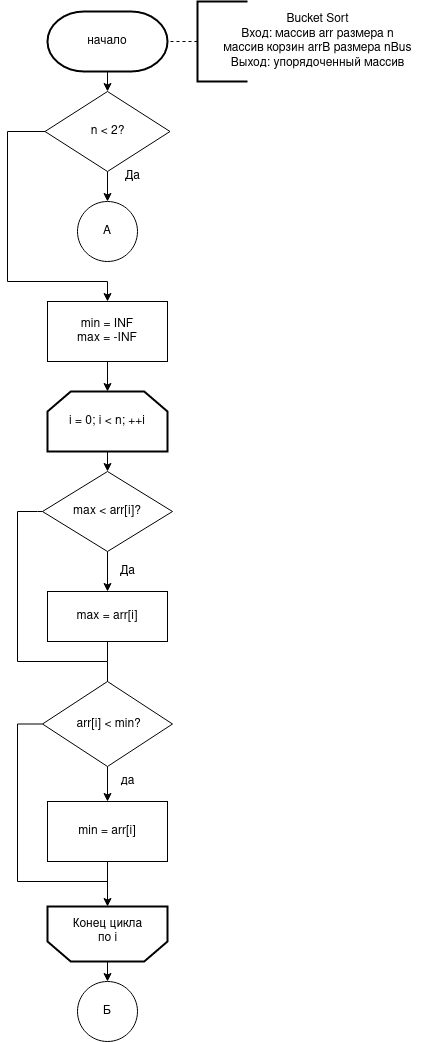
\includegraphics[width=0.32\linewidth]{bucket_1}
		\caption{Схема карманной сортировки, ч.1}
		\label{fig:schema_bucket_1}
	\end{figure}
	
	\begin{figure}[H]
		\centering
		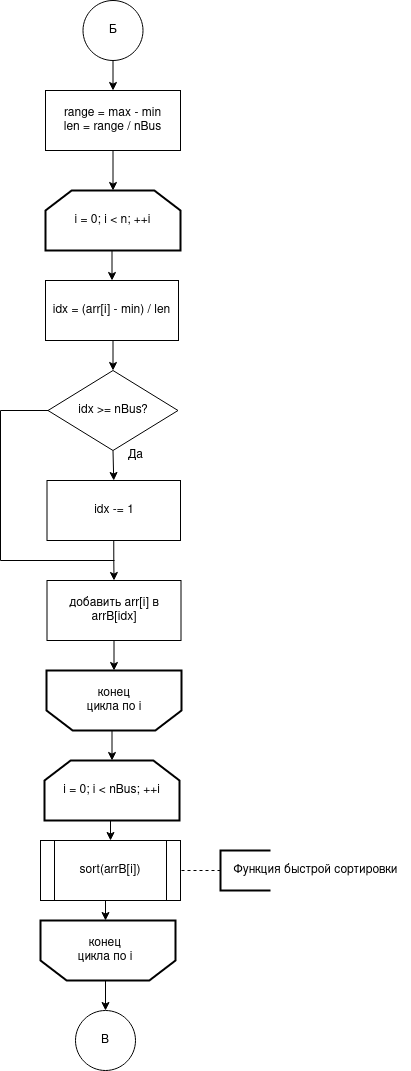
\includegraphics[width=0.5\linewidth]{bucket_2}
		\caption{Схема карманной сортировки, ч.2}
		\label{fig:schema_bucket_2}
	\end{figure}
	
	\begin{figure}[H]
		\centering
		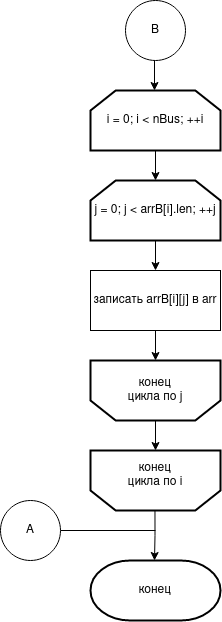
\includegraphics{bucket_3}
		\caption{Схема карманной сортировки, ч.3}
		\label{fig:schema_bucket_3}
	\end{figure}
	
	\begin{figure}[H]
		\centering
		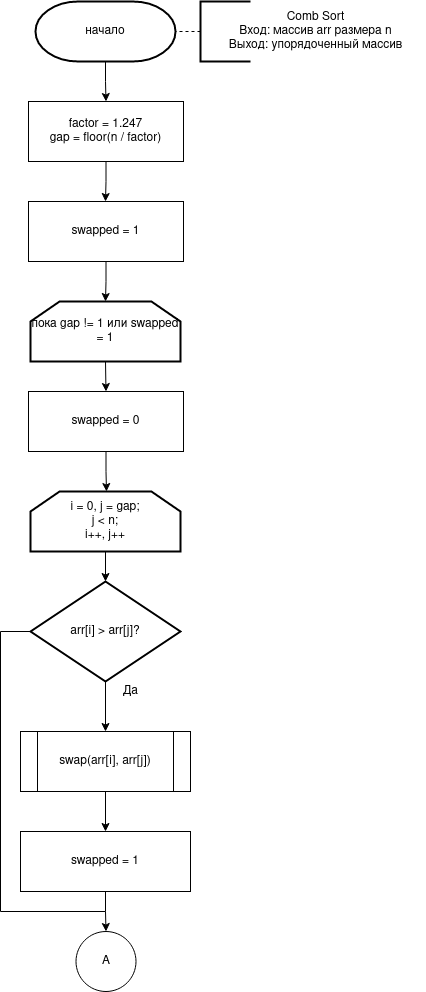
\includegraphics[width=0.5\linewidth]{combSort_1}
		\caption{Схема сортировки расческой, ч.1}
		\label{fig:schema_selection}
	\end{figure}
	
	\begin{figure}[H]
		\centering
		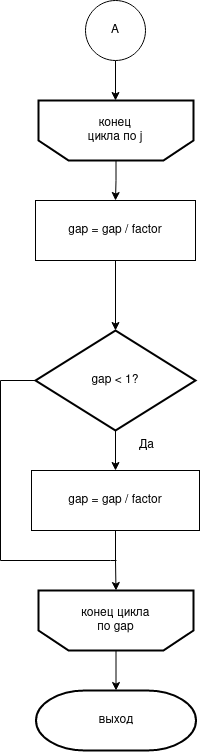
\includegraphics[width=0.35\linewidth]{combSort_2}
		\caption{Схема сортировки расческой, ч.2}
		\label{fig:schema_selection}
	\end{figure}
	
	\begin{figure}[H]
		\centering
		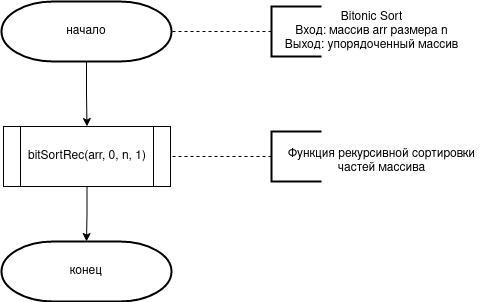
\includegraphics{bitonic_1}
		\caption{Схема основной функции алгоритма битонной сортировки}
		\label{fig:schema_insertion}
	\end{figure}
	
	\begin{figure}[H]
		\centering
		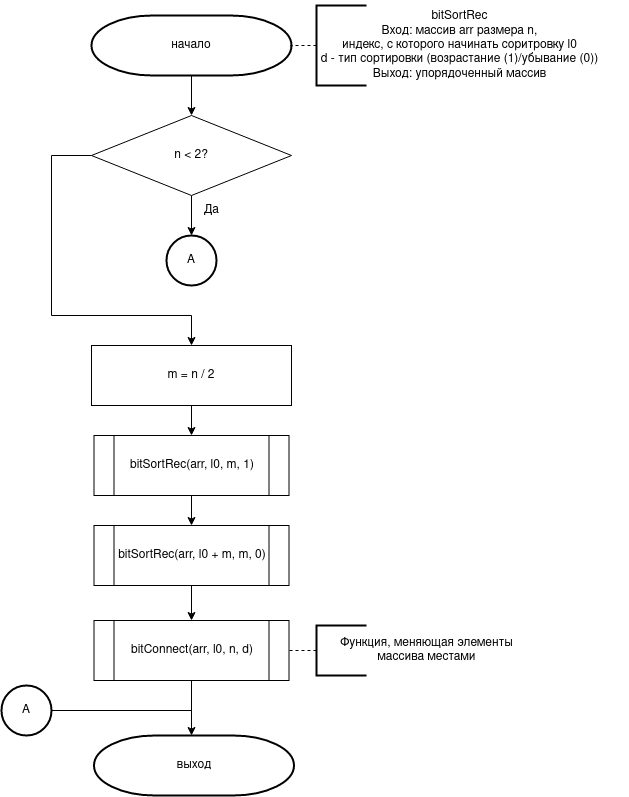
\includegraphics[width=0.9\linewidth]{bitonic_2}
		\caption{Схема процедуры bitSortRec алгоритма битонной сортировки}
		\label{fig:schema_insertion}
	\end{figure}
	
	\begin{figure}[H]
		\centering
		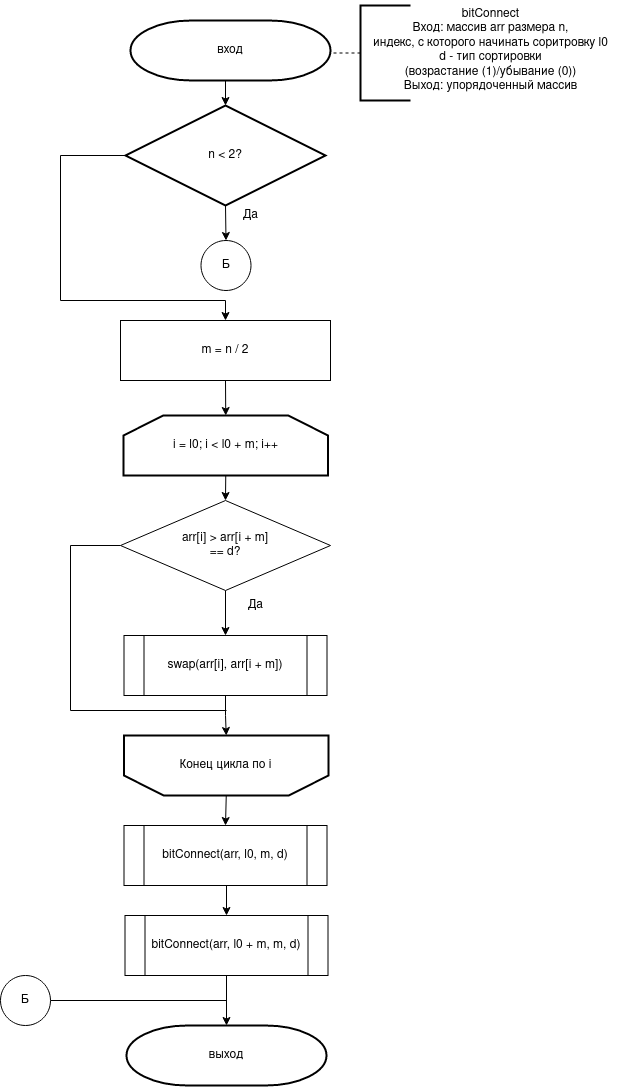
\includegraphics[width=0.7\linewidth]{bitonic_3}
		\caption{Схема процедуры bitConnect алгоритма битонной сортировки}
		\label{fig:schema_insertion}
	\end{figure}
	
	\section*{Вывод}
	
	В данном разделе на основе теоретических данных, полученных в аналитическом разделе были разработаны описания алгоримов трех рассматриваемых алгоритмов сортировок.
	
	\chapter{Технологическая часть}
	
	В данном разделе приведены требования к ПО, обоснования выбора языка программирования, среды разработки, приведен способ замера времени выполнения, а также приведены листинги кода.
	
	\section{Требования к ПО}
	
	В программе должна присутствовать возможность:
	
	\begin{enumerate}
		\item[1)] указания размера входного массива, а также его элементов;
		\item[2)] сортировки входного массива одним из трех рассматриваемых способов сортировок;
		\item[3)] замер процессорного времени выполрнения реализаций алгоритмов сортировки.
	\end{enumerate}
	
	\section{Выбор языка программирования и среды разработки}
	
	Для реализации трех алгоритмов сортировок был выбор язык С, так как я уже имею опыт разработки на данном языке программирования.

	Средой разработки был выбран СLion. Данный выбор обусловлен тем, что данная среда предоставляет возможность разработки приложений под с/c++ и имеет инструменты для отладки кода. 
	
	\section{Выбор библиотеки и способа для замера времени}
		Для замера времени выполнения сортировок использовалась стандартная функция библиотеки <time.h> языка С~---~clock(), которая замеряет процессорное время. Если измерить время перед началом выполнения алгоритма, и после его окончания, то можно получить время выполнения функции. Реализация данной функции приведена в [1].
		
		Поскольку все процессорное время не отдается какой-либо одной задаче (в связи с явлением вытеснения процессов из ядра, квантование процессорного времени), то требуется усреднить результаты вычислений: замерить совокупное время выполнения реализации алгоритма N раз и вычислить среднее время выполнения.
		
	\section{Реализации алгоритмов}
	
	В листингах \ref{bubble-code},\ref{selection-code},\ref{insertion-code} приведены реализации алгоритмов карманной, битонной сортировок и сортировки расческой  соответсвенно.
	
	\begin{lstlisting}[label=bubble-code,caption=Листинг карманной сортировки,language=C]
		void pushBackBucket(bucket *b, sortElem *e)
		{
		    b->arr[b->len] = *e;
		    (b->len)++;
		}

		void bucketSort(sortElem *arr, size_t n)
		{
		    if (n < 2)
			return clock() - timeStart;

		    sortElem min = { INF, DEFAULT_C, DEFAULT_D };
		    sortElem max = { -INF, DEFAULT_C, DEFAULT_D };
		    for (size_t i = 0; i < n; ++i) {
			if (comparatorIncrease(&max, arr + i))
			    max = arr[i];
			if (comparatorIncrease(arr + i, &min))
			    min = arr[i];
		    }

		    double range = (max.val) - min.val;
		    double lengthBucket = range / nBus;

		    for (size_t i = 0; i < n; ++i) {
			size_t idxBucket = (int)((arr[i].val - min.val) / lengthBucket);
			idxBucket = idxBucket >= nBus ? idxBucket - 1 : idxBucket;
			pushBackBucket(arrB + idxBucket, arr + i);
		    }

		    for (size_t i = 0; i < nBus; ++i)
			qsort(arrB[i].arr, arrB[i].len, sizeof(sortElem), comparatorIncrease);

		    size_t idx = 0;
		    for (size_t i = 0; i < nBus; ++i)
			for (size_t j = 0; j < arrB[i].len; ++j)
			    arr[idx++] = arrB[i].arr[j];
		}
	\end{lstlisting}

	
	\begin{lstlisting}[label=selection-code,caption=Листинг битонной сортировки,language=C]
		void compare(sortElem *arr, size_t i, size_t j, int d)
		{
		    if (d == comparatorIncrease(arr + i , arr + j))
		    {
			sortElem tmp = arr[i];
			arr[i] = arr[j];
			arr[j] = tmp;
		    }
		}

		void bitonicConnect(sortElem* arr, size_t lo, size_t n, int d)
		{
		    if (n < 2)
			return;

		    size_t m = n / 2;
		    for (size_t i = lo; i < lo + m; ++i)
		    {
			compare(arr, i, i + m, d);
		    }
		    bitonicConnect(arr, lo, m, d);
		    bitonicConnect(arr, lo + m, m, d);
		}

		void bitonicSortRecursive(sortElem *arr, size_t lo, size_t n, int dir)
		{
		    if (n < 2)
			return;

		    size_t m = n / 2;
		    bitonicSortRecursive(arr, lo, m, INC);
		    bitonicSortRecursive(arr, lo + m, m, DEC);
		    bitonicConnect(arr,lo, n, dir);
		}

		void bitonicSort(sortElem *arr, size_t n)
		{
		    bitonicSortRecursive(arr, 0, n, INC);
		}
	\end{lstlisting}
	
	\bigbreak

	\begin{lstlisting}[label=insertion-code,caption=Листинг сортировки расческой,language=C]
		void combSort(sortElem *arr, size_t n)
		{
		    float factor = 1.247f;
		    size_t gap = (size_t)(n / factor);
		    int swapped = 1;
		    while (gap != 1 || swapped) {
			swapped = 0;
			for(size_t i = 0, j = gap; j < n; ++i, ++j)
			{
			    if (comparatorIncrease(arr + i, arr + j)) {
				sortElem tmp = arr[i];
				arr[i] = arr[j];
				arr[j] = tmp;
				swapped = 1;
			    }
			}
			gap = gap / factor < 1 ? 1 : gap / factor;
		    }
		}
	\end{lstlisting}

	\section{Тестирование алгоритмов}

	В таблице~\ref{tbl:test} приведены тесты для функций, реализующих алгоритмы сортировки. Все тесты пройдены успешно.
	
	\begin{table}[h!]
		\begin{center}
			\caption{\label{tbl:test}: Тестирование функций}
			\begin{tabular}{|c|c|c|}
				\hline
				Входной массив & Результат & Ожидаемый результат \\ 
				\hline
				$[10, 20, 30, 40, 50]$ & $[10, 20, 30, 40, 50]$  & $[10, 20, 30, 40, 50]$\\\hline
				$[50, 40, 30, 20, 10]$  & $[10, 20, 30, 40, 50]$ & $[10, 20, 30, 40, 50]$\\\hline
				$[-15, -21, -37, -24, -54]$  & $[-54, -37, -24, -21, -15]$  & $[-54, -37, -24, -21, -15]$\\\hline
				$[4]$  & $[4]$  & $[4]$\\\hline
				Пустой массив  & Пустой массив  & Пустой массив\\
				\hline
			\end{tabular}			
		\end{center}
	\end{table}

	\section*{Вывод}
	
	В данном разделе были разработаны исходные коды трёх алгоритмов сортировок: расческой, битонной и карманной.
	
	\chapter{Экспериментальная часть}
	
	\section{Технические характеристики}
	
	Ниже приведены технические характеристики устройства, на котором было проведено тестирование ПО:
	
	\begin{enumerate}
		\item[1)] операционная система Windows-10, 64-bit;
		\item[2)] оперативная память 16 ГБ;
		\item[3)] процессор Intel(R) Core(TM) i7-8565U CPU @ 1.80 Ггц, 4 ядра, 8 логических процессоров.
	\end{enumerate}
	
	\section{Замеры времени}
	
	Введем обозначения: comb -- алгоритм сортировки расческой, bucket - алгоритм карманной сортировки, bitonic - алгоритм битонной сортировки. 
	
	В таблице \ref{table:t1} приведены результаты замеров времени для лучшего случая работы алгоритмов.
	
	\begin{table} [H]
		\caption{Таблица замера времени выполнения сортировок на данных, отсоритрованных по возрастанию (в мс)}
		\label{table:t1}
		\begin{center}
			\begin{tabular}{|c | c | c | c|}
				
				\hline
				
				Размер & comb & bucket & bitonic  \\ [0.5ex]
				
				\hline
				
				100 & 7.8 & 7.61 & 27.3 \\ 
				
				\hline 
				
				1000 & 113 & 100.4 & 428.1 \\ 
				
				\hline 
				
				10000 & 1750 & 801.57 & 12427.6 \\ 
				
				\hline 
			\end{tabular}
		\end{center}
	\end{table}

	Зависимость времени от количества элементов для лучшего случая работы алгоритмов представлена на рис. \ref{ris1}.

	\begin{center}
		\begin{figure}[H]
		\center
		\begin{tikzpicture}
				\begin{axis} [
					legend pos = north west,
					grid = major,
					xmin = 0,
					ymin = 0, 
					xmax = 10000,
					ymax = 13000,
					xlabel = $\text{количество элементов}$,
					ylabel = $\text{время (мс)}$
					]
					\legend{ 
						$comb$, 
						$bucket$, 
						$bitonic$
					};
					\addplot coordinates {
						(100,7.08) (1000,113) (10000,1750)
					};
					\addplot coordinates {
						(100,7.61) (1000,100.4) (10000,801.57)
					};
					\addplot coordinates {
						(100,27.3) (1000,428.1) (10000,12427.6)
					};
				\end{axis}
		\end{tikzpicture}
		\caption{Зависимость времени от количества элементов}
		\label{ris1}
		\end{figure}
	\end{center}
	
	В таблице \ref{table:t2} приведены результаты замеров времени для худшего случая работы алгоритмов:
	
	\begin{table} [H]
		\caption{Таблица замера времени выполнения сортировок на данных, отсоритрованных по убыванию (в мс)}
		\label{table:t2}
		\begin{center}
			\begin{tabular}{|c | c | c | c|}
				
				\hline
				
				Размер & comb & bucket & bitonic  \\ [0.5ex]
				
				\hline
				
				100 & 9.6 & 7.71 & 28.49 \\ 
				
				\hline 
				
				1000 & 130.27 & 96.4 & 390.85 \\ 
				
				\hline 
				
				10000 & 2066.09 & 888.5 & 11475.05 \\ 
				
				\hline 
				
			\end{tabular}
		\end{center}
	\end{table}
	
	Зависимость времени от количества элементов для худшего случая работы алгоритмов представлена на рис. \ref{ris2}.

	\begin{center}
		\begin{figure}[H]
		\center
		\begin{tikzpicture}
			\begin{axis} [
				legend pos = north west,
				grid = major,
				xmin = 0,
				ymin = 0, 
				xmax = 10000,
				ymax = 13000,
				xlabel = $\text{количество элементов}$,
				ylabel = $\text{время (мс)}$
				]
				\legend{ 
					$comb$, 
					$bucket$, 
					$bitonic$
				};
				\addplot coordinates {
					(100,9.6) (1000,130.27) (10000,2066.09)
				};
				\addplot coordinates {
					(100,7.71) (1000,96.4) (10000,888.5)
				};
				\addplot coordinates {
					(100,28.49) (1000,390.85) (10000,11475.05)
				};
			\end{axis}
		\end{tikzpicture}
		\caption{Зависимость времени от количества элементов}
		\label{ris2}
		\end{figure}
	\end{center}
	
	В таблице \ref{table:t3} приведены результаты замеров времени работы алгоритмов на случайно заполненном массиве:
	
	\begin{table} [h!]
		\caption{Таблица замера времени выполнения сортировок на случайных данных (от 0 до 1000) (в мс)}
		\label{table:t3}
		\begin{center}
			\begin{tabular}{|c | c | c | c|}
				
				\hline
				
				Размер & comb & bucket & bitonic  \\ [0.5ex]
				
				\hline
				
				100 & 12.38 & 12.78 & 39.79 \\ 
				
				\hline 
				
				1000 & 189.44 & 189.77 & 486.02 \\ 
				
				\hline 
				
				10000 & 2491.19 & 1975.79 & 12273.07 \\ 
				
				\hline 
				
			\end{tabular}
		\end{center}
	\end{table}

	Зависимость времени от количества элементов для работы алгоритмов на случайно заполненном массиве представлена на рис. \ref{ris3}.
	
	\begin{center}
		\begin{figure}[H]
		\center
		\begin{tikzpicture}
			\begin{axis} [
				legend pos = north west,
				grid = major,
				xmin = 0,
				ymin = 0, 
				xmax = 10000,
				ymax = 13000,
				xlabel = $\text{количество элементов}$,
				ylabel = $\text{время (мс)}$
				]
				\legend{ 
					$comb$, 
					$bucket$, 
					$bitonic$
				};
				\addplot coordinates {
					(100,12.38) (1000,189.44) (10000,2491.19)
				};
				\addplot coordinates {
					(100,12.78) (1000,189.77) (10000,1975.79)
				};
				\addplot coordinates {
					(100,39.79) (1000,486.02) (10000,12273.07)
				};
			\end{axis}
		\end{tikzpicture}
		\caption{Зависимость времени от количества элементов}
		\label{ris3}
		\end{figure}
	\end{center}
	
	В таблице \ref{table:t4} приведены результаты замеров времени работы алгоритмов на случайно заполненном массиве:
	
	\begin{table} [H]
		\caption{Таблица времени выполнения сортировок на случайных данных (от 0 до 3) (в мс)}
		\label{table:t4}
		\begin{center}
			\begin{tabular}{|c | c | c | c|}
				
				\hline
				
				Размер & comb & bucket & bitonic  \\ [0.5ex]
				
				\hline
				
				100 & 8.89 & 8.08 & 31.94 \\ 
				
				\hline 
				
				1000 & 100.6 & 100.66 & 405.61 \\ 
				
				\hline 
				
				10000 & 1763.35 & 1286.04 & 11061.61 \\ 
				
				\hline 
				
			\end{tabular}
		\end{center}
	\end{table}
	
	Зависимость времени от количества элементов для работы алгоритмов на случайно заполненном массиве представлена на рис. \ref{ris4}.
	
	\begin{center}
		\begin{figure}[H]
		\center
		\begin{tikzpicture}
			\begin{axis} [
				legend pos = north west,
				grid = major,
				xmin = 0,
				ymin = 0, 
				xmax = 10000,
				ymax = 13000,
				xlabel = $\text{количество элементов}$,
				ylabel = $\text{время (мс)}$
				]
				\legend{ 
					$comb$, 
					$bucket$, 
					$bitonic$
				};
				\addplot coordinates {
					(100,8.89) (1000,100.6) (10000,1763.35)
				};
				\addplot coordinates {
					(100,8.08) (1000,100.66) (10000,1286.04)
				};
				\addplot coordinates {
					(100,31.94) (1000,405.61) (10000,11061.61)
				};
			\end{axis}
		\end{tikzpicture}
		\caption{Зависимость времени от количества элементов}
		\label{ris4}
		\end{figure}
	\end{center}
	

	\section*{Вывод}
	
	Результаты замеров показали, что алгоритм карманной сортировки, который сортирует корзины быстрой сортировкой, работает быстрее на случайно отсортированном массиве с элементами от 0 до 1000, чем сортировка битонная сортировка  (так как массив из 10000 элементов дополняется до $2^N$) и сортировка расческой (так как быстрая сортировка в модификации может сортировать элементы за $O(N)$ при делении массива на 3 части). При этом карманная сортировка работает быстрее на предварительно отсортированных массивах, чем на случайным образом заполненных массивах, (при условии, что количество корзин берется как $0.5 \cdot N$), так как в этом случае меньше элементов попадает в одну и ту же корзину. 
	
	\chapter*{Заключение}
	
	Цель работы достигнута: выполнено исследование алгоритмов сортировок расческой, карманной и битонной. Все задаче решены:
	
	\begin{enumerate}
		\item[1)] были изучены и рассмотрены алгоритмы сортировок пузырьком, вставками и выбором;
		\item[2)] были построены блок-схемы выбранных алгоритмов;
		\item[3)] был реализован каждый из алгоритмов;
		\item[4)] была рассчитана их трудоемкость;
		\item[5)] были экспериментально получены временные характеристики алгоритмов;
		\item[6)] были сделаны выводы на основании проделанной работы
	\end{enumerate}
	
	На основании анализа трудоемкости алгоритмов в выбранной модели вычислений, было показано, что алгоритм карманной сортировки с количеством выбираемых карманов $0.5 \cdot N$ и алгоритмом быстрой сортировки карманов эффективнее работает на отсортированных по возрастанию/убыванию массивах (нежели на случайно отсортированных), обгоняя по скорости алгоритмы битонной сортировки и сортировки расческой.
	
\addcontentsline{toc}{chapter}{Список использованных источников}

\nocite{*} 

\renewcommand\bibname{Список использованных источников} % переименовать страницу списка литературы
\bibliographystyle{utf8gost705u}  % стилевой файл для оформления по ГОСТу
\bibliography{lib}          % имя библиографической базы (bib-файла)
	
\end{document}
